\documentclass{article}[12pt]
\usepackage{fullpage}
% Packages
\usepackage{amsfonts}
\usepackage{amsmath}
\usepackage{amsthm}
\usepackage{graphicx}


\theoremstyle{plain}
\newtheorem{lemma}{Lemma}
\newtheorem{claim}[lemma]{Claim}
\newtheorem{theorem}[lemma]{Theorem}
\newtheorem{corollary}[lemma]{Corollary}
\newtheorem{definition}{Definition}

\newcommand{\note}[1]{\par{\bf Note:}#1\par}
\newcommand{\notem}[1]{{\marginpar{\tiny #1}}}

\newcommand{\figline}{\rule{\textwidth}{1pt}}

%\newcommand{\proof}{\noindent{\bf Proof:} }
%\newcommand{\qed}{\rule{0.7em}{0.7em}}

\newcommand{\newmcommand}[2]{\newcommand{#1}{{\ifmmode {#2}\else\mbox{${#2}$}\fi}}}
\newcommand{\newmcommandi}[2]{\newcommand{#1}[1]{{\ifmmode {#2}\else\mbox{${#2}$}\fi}}}
\newcommand{\newmcommandii}[2]{\newcommand{#1}[2]{{\ifmmode {#2}\else\mbox{${#2}$}\fi}}}
\newcommand{\newmcommandiii}[2]{\newcommand{#1}[3]{{\ifmmode {#2}\else\mbox{${#2}$}\fi}}}

\newcommand{\E}[2]{{\bf E}_{#1}\left[ #2 \right]}
\newcommand{\reals}{\mathbb{R}}

\newcommand{\R}{R}      % Cumulative regret
\renewcommand{\r}{r}      % Instantaneuous regret
\newcommand{\state}{{\bf \Psi}}
\newcommand{\finalPot}{\Phi_{\mbox{T}}}
\newcommand{\pot}{\Phi}
\newcommand{\upperpot}{\Phi^{\downarrow}}
\newcommand{\lowerpot}{\Phi^{\uparrow}}
\newcommand{\score}{\phi}
\newcommand{\learnerM}{P}
\newcommand{\adversM}{Q}
\newcommand{\agloss}{v}
\newcommand{\Bias}{B}

\newmcommandi{\paren}{\left({#1}\right)}




\title{Strategies for convex potential games \\
  and an application to
  decision-theoretic online learning}
\author{Yoav Freund}
\begin{document}
\maketitle
\begin{abstract}
The backwards induction method due to Bellman~\cite{bellman1952theory}
is a popular approach in optimiztion, optimal control, and many other
areas of applied math. In this paper we analyze the backwords
induction approach, under min/max conditions. We show that if the
value function is has strictly positive derivatives of order 1-4 then
the optimal strategy for the adversary is brownian motion. Using that
fact we analyze different potential functions and show that the
Normal-Hedge potential is optimal.
\end{abstract}

\section{Introduction}

Our analysis is an application of Bellman's
equation~\cite{bellman1952theory} and the more recent work on drifting
games by Schapire\cite{schapire2001drifting}.
This setup has been studied
in the past (BW algorithm, drifting games).

We describe a set of strategies for the decision-theoretic online
learning problem (DTOL)~\cite{}. To develop those strategies we
replace discrete time: $t=0,1,2,\ldots,T$ with
continuous time: $t \in [0,T]$. Suppose there are $N$ actions whose per iteration
loss is in the range $[0,1]$, and suppose that the game is repeated
$T$ times. There are several algorithm whose regret is bounded by
$C\sqrt{T \ln N}$ for some constant $C$. Next Suppose that the
actual losses are in the range $[0,1/2]$ which would imply that the
regret is at most $\frac{C}{2}\sqrt{T \ln N}$ and that the bound is
twice large than it should be. We will show that a natural way to
remove this slack is to say that time increases in increments of
$1/4$ so that the final time is $T/4$. In this paper we show that this
idea is very general and leads to a a min/max optimal algorithm for DTOL.


\section{Setup}
The game takes place on the set $(t,\R) \in [0,T] \times \reals$,
where $t$ corresponds to time, $T$ correspond to the
end time of the game (i.e. this is a bounded horizon game where the
horizon is known to both players. $\R$ curresponds to (total) regret.

We will first consider the standard setting where time corresponds to
the natural and is equal to the iteration number $t_i=i$. Later we
expand the game the $t_i$ can take on any real value in $[0,T]$ under
the ccondition that $t_{i-1} \leq t_i \leq t_{i-1}+1$.

The {\em state} of the game at time $t_i$ is a distribution over regrets 
$\reals$ denoted by $\R \sim \state(t_i)$. The initial distribution $\state(0)$
is delta-function at $\R=0$. States $\state(t_i)$ for $t>0$ also
correspond to distributions over regret.
The state $\state(t)$ is defined by $\state(t_{i-1})$ and the choices made
by the two players as described in the next section.

There are two players: the {\em learner} and the {\em adversary}. There is a
value function defined for the final state
$\finalPot = \pot(T):\reals \to \reals$.

The final potential $\finalPot(\R)$ is fixed a-priori and is known to
both players. $\finalPot(\R)$ is restricted to be  continuous, monotone
non-decreasing and strictly convex. We will refer to these conditions
as {\bf CIC}.

The outcome of the game is the expected final value,
\begin{equation} \label{eqn:FinalExpectedValue}
  \score(T) =\E{\R \sim \state(T)}{\finalPot(\R)}
\end{equation}

The goal of the learner is to minimize $\score(T)$ and the goal of
the adversary is to maximize it.

\section{Integer time game}
We start with the standard setup in which time corresponds to the
natural numbers, $t_i=i$. to simplify notation we will use the
iteration number $i$ instead of time.

Connecting this back to decision theoretic online learning
(DTOL~\cite{}). The state $\state(i)$ corresponds to the distribution
over the regret values of the experts on iteration $i$. Note that here the set of
experts is allowed to be be uncountably infinite. In particular the
adversary can assign to the experts with regret $x$ at iteration $t$
an arbitrary distribution of losses in the range $[-1,+1]$.

The game is defined by three parameters:
\begin{itemize}
\item $T$ : The number of iterations
\item $\finalPot(\R)$ : The final value function that is CIC.
\item $0<c \leq 1$ - An upper bound on aggregate loss (loss of the master)
  in a single iteration. Note that the cumulative aggregate loss is at
  most $cT$. Note that $c=1$ is always satisfied and nullifies the
  constraint.
\end{itemize}

The transition from $\state(i)$ to $\state(i+1)$ is  defined by the
choices made by the adversary and the learner.

\begin{enumerate}
\item The learner chooses weights. Formally, this is
  a distribution over $\R \in \reals$: $\learnerM(i)$.
\item The adversary chooses the losses of the actions. Formally 
  this is a mapping from $\reals$ to distributions
  over $[-1,+1]$: $\adversM(i): \reals \to \Delta^{[-1,+1]}$. We use
  $l \sim \adversM(i,\R)$ to denote the distribution over the
  instantanous loss associated with iteration $i$ and regret $\R$.
\item The aggregate loss (also called ``the loss of the master") is
  calculated:
  \begin{equation} \label{eqn:agg-loss-complex}
  \ell(i)=\E{\R \sim \state(i)}{\learnerM(i,\R) \E{l \sim \adversM(i,\R)}{l}}
  \end{equation}
  
  The adversary is constrained to $\adversM$ such $|\ell(i)| \leq c$. 
  We define the {\em bias} at $(i,\R)$ to be  $\Bias(i,\R) \doteq \E{l
    \sim \adversM(i,\R)}{l}$ which allows us to rewrite
  Eqn~(\ref{eqn:agg-loss-complex}) as
  
  \begin{equation} \label{eqn:aggregate-loss}
    \ell(i)=\E{\R \sim \state(i)}{\learnerM(i,\R) \Bias(i,\R)}
  \end{equation}
  note that $\Bias(i,\R)$ is in $[-1,1]$ and that $\ell(i)$ is the mean
  of $\Bias(i,\cdot)$. Note also that $-1-c \leq y-\ell(i) \leq 1+c$
  corresponds to the instantanous regret. In the integer game, setting
  $c \geq 1$ is equivalent to placing no restriction on $\ell(i)$.
  
\item The state is updated. 
  \begin{equation} \label{eqn:state-update}
    \state(i+1) = \E{\R \sim \state(i)}{\R \oplus  \adversM(i,\R)}
    \ominus \ell(i)
    \end{equation}
  Where $\adversM(i,\R)$ is the distribution of the losses of experts
  that are at location $\R$ after iteration $i-1$. $\R \oplus
  \adversM(i,\R)$ is the same distribution shiften right by the amount
  $\R$. $ \E{\R \sim  \state(i-1)}{\cdot}$ indicates the expectation over distribution,
  yealding a new distribution. Finally $\ominus \ell(i)$ is a shift
  left of the resulting distribtion according to the aggregate loss. 
\end{enumerate}

The final outcome of the game is given in
Equation~(\ref{eqn:FinalExpectedValue}).

\subsection{Strategies for integer time game}

Consider the states at two consecutive iterations $\state(i-1),\state(i)$.
Suppose that $\pot(i,\R)$, the value function for iteration $i$ is fixed.
We say that $\lowerpot(i-1,\R)$ is a lower bound on the value at iteration
$i-1$ if there is exists an adversarial strategy $\adversM^*$ such that
for any strategy of the learner $\learnerM$, 
$$ \E{\R \sim \state(i-1)}{\lowerpot(i-1)} \leq \E{\R \sim \state(i)}{\pot(i)}$$
Similarly, $\upperpot(i-1,\R)$ is an upper potential if there exists a
learner strategy $\learnerM^*$ such that for any adversarial strategy
$\adversM$,
$$ \E{\R \sim \state(i-1)}{\upperpot(i-1)} \geq \E{\R \sim \state(i)}{\pot(i)}$$


\begin{lemma} \label{lemma:adversary-prefers-extremes}
 Suppose $\lowerpot(i,\R)$ is strictly convex with respect to  $\R$.
Let ${\cal Q}(i-1,\R,\Bias)$ be the set of adversarial strategies 
$\adversM(i-1,\R)$ that have bias
$\Bias=\Bias(i-1,\R)= \E{y \sim \adversM(i-1,\R)}{y}$ then the
strategy in ${\cal Q}(i-1,\R,\Bias)$ that is best for the adversary is
\begin{equation} \label{eqn:adv-strat-p}
  \adversM^p(i-1,\R) =
  \begin{cases}
    +1 & \mbox{ w.p. } \frac{1+\Bias}{2}\\
    -1 & \mbox{ w.p. } \frac{1-\Bias}{2}\\
  \end{cases}
\end{equation}

\begin{equation} \label{eqn:value-iteration-lower}
  \lowerpot(i-1, \R) = p \lowerpot(i,\R+1) + (1-p)\lowerpot(i,\R-1)
\end{equation}
which is strictly higher than $\lowerpot(i-1,\R)$ for any other
distribution in ${\cal Q}(i-1,\R,\Bias)$. In addition,
$\lowerpot(i-1, \R)$ is strictly convex.
\end{lemma}


In the next lemma we describe strategies for the adversary and the
learner and prove upper and lower bounds on the potential that they
guarantee.

\begin{lemma} \label{lemma:first-order-bound}
  If $\pot(i,\R)$  is CIC then
  \begin{enumerate}
    \item The adversarial strategy
      \begin{equation} \label{eqn:adv-strat}
      \adversM^{1/2}(i-1,\R) =
      \begin{cases}
        -1 & \mbox{ w.p. } 1/2\\
        +1 & \mbox{ w.p. } 1/2
      \end{cases}
    \end{equation}
    Guarantees the lower potential
 \begin{equation} \label{eqn:value-iteration-lower}
   \lowerpot(i-1, \R) = \frac{\pot(i,\R+1) + \pot(i,\R-1)}{2}
 \end{equation}
   
    \item The learner strategy:
      \begin{equation} \label{eqn:learner-strat-1}
      \learnerM^1(i-1,\R) = \frac{1}{Z} \frac{\pot(i,\R+1+c) - \pot(i,\R-1-c)}{2}
      \end{equation}
      Where $Z$ is a normalization factor
      $$Z = \E{\R \sim \state(i)}{\frac{\pot(i,\R+1+c) - \pot(i,\R-1-c)}{2}}$$
      guarantees the upper potential 
      \begin{equation} \label{eqn:value-iteration-upper}
        \upperpot(i-1, \R) = \frac{\pot(i,\R+1+c) + \pot(i,\R-1-c)}{2}
      \end{equation}
    \end{enumerate}
    
\end{lemma}


\proof ~\\
\begin{enumerate}
\item By symmetry adversarial strategy~(\ref{eqn:adv-strat}) guarantees that
  the aggregate loss~(\ref{eqn:aggregate-loss}) is zero regardless of
  the choice of the learner: $\ell(t)=0$.
  Therefor the state update~(\ref{eqn:state-update}) is equivalent to
  the symmetric random walk:
  $$\state(i) = \frac{1}{2} \paren{(\state(i-1) \oplus 1) + (\state(i-1)
    \ominus 1)}$$
  Which in turn implies that if the adversary plays $\adversM^*$
  and the learner plays an arbitrary strategy $\learnerM$
  \begin{equation} \label{eqn:lower}
    \lowerpot(i-1,\R) = \frac{1}{2} \paren{\pot(i,\R-1)+\pot(i,\R+1)}
  \end{equation}
  As this adversaril strategy is oblivious to the strategy, it
  guarantees that the average value at iteration $i$ is {\em equal} to the
  average of the lower value at iteration $i-1$.
\item
 Plugging learner's strategy~(\ref{eqn:learner-strat-1}) into equation~(\ref{eqn:aggregate-loss}) we find that
 \begin{equation} \label{eqn:ell-optimal-learner}
   \ell(i-1) = \frac{1}{Z_{i-1}} \E{\R \sim \state(i-1)}{\paren{\pot(i,\R+1+c)-\pot(i,\R-1-c)}
   \Bias(i-1,\R)}
\end{equation}
  Consider the average value at iteration $i-1$ when the learner's strategy
  is $\learnerM^*$ and the adversarial strategy is arbitrary $\adversM$:
  
   \begin{equation} \label{eqn:Pot-Update}
    \score_{\learnerM^*,\adversM}(i-1,\R) = \E{\R \sim \state(i-1)}{ \E{y \sim
      \adversM(i-1)(\R)}{\pot(i,\R+y-\ell(i-1))}}
  \end{equation}
  As $\pot(i,\cdot)$ is convex and as $(y-\ell(i-1)) \in [-1-c,1+c]$,
  \begin{equation} \label{eqn:pot-upper}
    \pot(i,\R+y) \leq \frac{\pot(i,\R+1+c)+\pot(i,\R-1-c)}{2} +
    (y-\ell(i)) \frac{\pot(i,\R+1+c)-\pot(i,\R-1-c)}{2}
    \end{equation}
  Combining the equations~(\ref{eqn:ell-optimal-learner}) and~(\ref{eqn:Pot-Update}) we find that
  \begin{eqnarray}
  \score_{\learnerM^*,\adversM}(i-1,\R)&=&\E{\R \sim \state(i-1)}{\E{y \sim \adversM(i-1)(\R)}{\pot(i,\R+y-\ell(i-1))}}\\
  &\leq & \E{\R \sim \state(i-1)}{\frac{\pot(i,\R+1+c)+\pot(i,\R-1-c)}{2}}\\
  &+&
  \E{\R \sim \state(i-1)}{\E{y \sim \adversM(i-1)(\R)}{(y-\ell(i-1)) \frac{\pot(i,\R+1+c)-\pot(i,\R-1-c)}{2}}} \label{eqn:zero-term}
  \end{eqnarray}
  
The final step is to show that the term~(\ref{eqn:zero-term}) is equal
to zero. As $\ell(i-1)$ is a constant with respect to $\R$ and $y$ the
term~(\ref{eqn:zero-term}) can be written as:
\begin{eqnarray}
&&\E{\R \sim \state(i-1)}{\E{y \sim \adversM(i-1)(\R)}{(y-\ell(i-1))
   \frac{\pot(i+1,\R+1)-\pot(i+1,\R-1)}{2}}}\\
&=&
\E{\R \sim \state(i-1)}{\Bias(i-1,\R)
    \frac{\pot(i,\R+1+c)-\pot(i,\R-1-c)}{2}}\\
  &-& \ell(i) \E{\R \sim \state(i-1)}{
    \frac{\pot(i,\R+1+c)-\pot(i,\R-1-c)}{2}}\\
  &=& 0
\end{eqnarray}
\end{enumerate}
\qed

  We find that the lower bound corredponds to an unbiased random
  walk with step size $\pm 1$. The upper bound also corresponds to a an
  unbiasd random walk with step size $\pm(1+c)$. The natural setting
  in the natural game is $c=1$, which means that there is a
  significant difference between the upper and lower bounds. As we
  show in the next section, this gap converges to zero in the
  continuous time setting, and the upper and lower bounds match,
  making the strategies for both sides min-max optimal. 

  Note also that the adversarial strategy the aggregate loss
  $\ell(t)$ is always zero, regardless of the strategy of the
  learner, and state progression is independent of the
  learner's choices.

  \begin{figure}[t]
%\vskip -0.2in
\begin{center}
\centerline{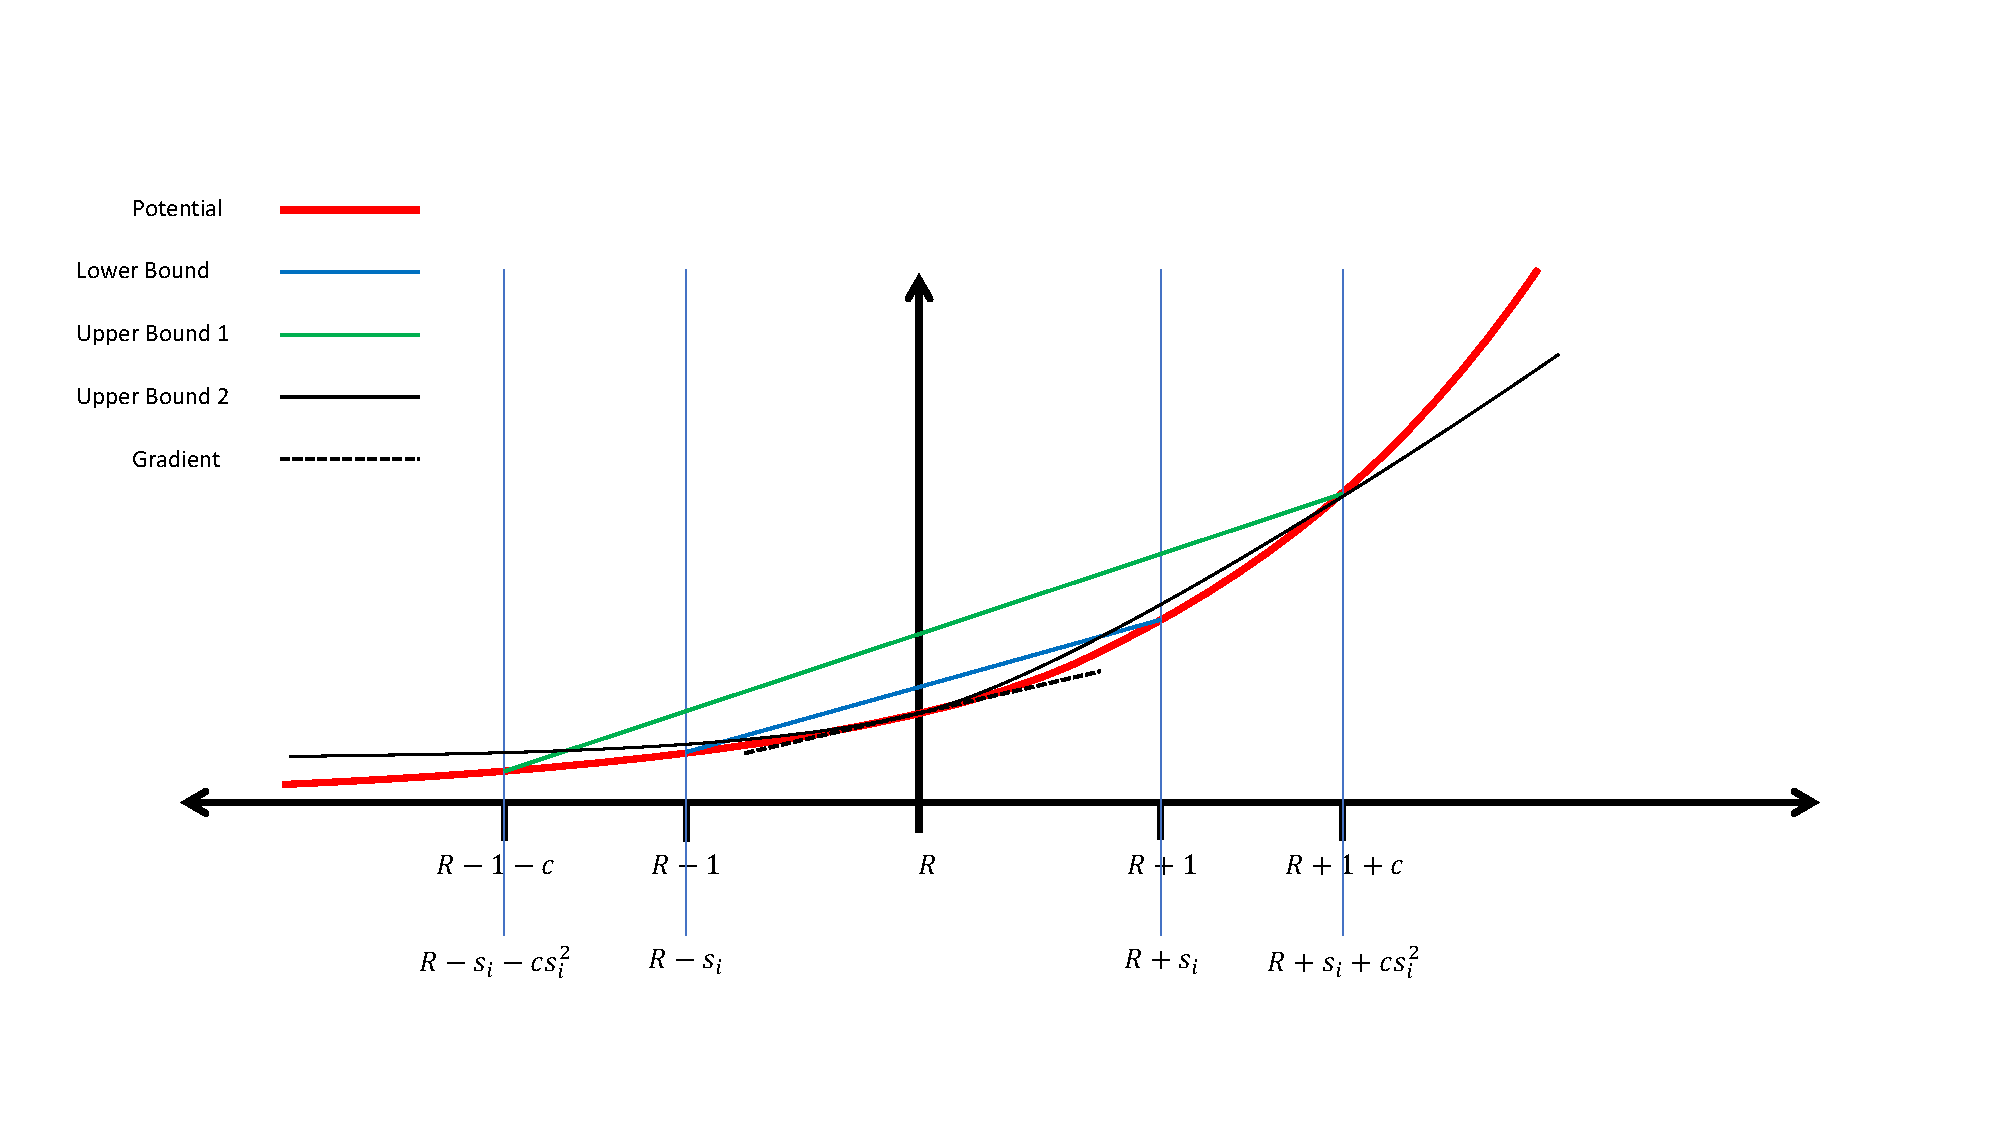
\includegraphics[width=\textwidth]{figures/convexPot.pdf}}
\caption{This figure depicts the relationship between the different
  upper and lower bounds used in the analysis. To aid understanding we
  describe the elements of the figure twice: once for the integer
  game, and once for the continuous time game. \newline
  {\bf Integer time game:} let
  the current iteration be $i$ and let the current regret be $\R$. Let
  $r$ be the regret at iteration $i+1$, we have that $\R-1-c \leq r
  \leq \R+1+c$. The
  potential at iteration $i+1$ is $\pot(i+1,r)$ (the red curve). The lower bound
  (blue line) corresponds to the adversarial strategy:
  $\adversM^{1/2}(i,\R)$. The first-order learner strategy:
  $\learnerM^1(i,\R)$ corresponds to the green line. The second-order
  learner strategy:  $\learnerM^2(i,\R)$ corresponds to the black
  curve.\newline
{\bf Continuous time game:} let
  the current iteration be $i$, the current time be $t_i$ and the
  current regret be $\R$. Let $0<s_i\leq 1$ be the step size chosen by the
  adversary, so that the next time is $t_{i+1} = t_i+s_i^2$. Let $r$
  be the regret at iteration
  $i+1$, we have that $\R-s_i-c s_i^2 \leq r \leq \R+s_i+c s_i^2$.
  The potential at iteration $i+1$ is $\pot(t_{i+1},r)$ (the red
  curve).  The lower bound (blue line) corresponds to the adversarial
  strategy: $\adversM^{1/2}_{\pm s_i}(t_i,\R)$. The first-order learner strategy:
  $\learnerM^{1c}(t_i,\R)$ corresponds to the green line. The second-order
  learner strategy: $\learnerM^{2c}(i,\R)$ corresponds to the black
  curve.   Observe that when $s_i \to 0$ the ratio $\frac{s_i}{s_i+c
    s_i^2}$ converges to 1, and the upper and gap between the green
  and blue lines converges to zero.\\
\rule[1ex]{6.5in}{0.5pt}}
\label{fig:ConvexPot}
\end{center}
\vskip -0.4in
\end{figure} 

  \subsection{A learner strategy with a variance-dependent bound}

  As shown in Lemma~\ref{lemma:adversary-prefers-extremes}, the
  adversary always prefers mixed strategies that assign zero
  probability for all steps other than $\pm 1$. Suppose, however, that
  the adversary is not worst-case optimal and chooses steps whose
  length is less than one. The following lemma gives a slightly
  different strategy for the learner, which guarantees a tighter bound
  for this case.

  \begin{lemma} \label{lemma:second-order-bound}
      The learner strategy:
      \begin{equation} \label{eqn:learner-strat-2}
      \learnerM^2(i-1,\R) =  \frac{1}{Z}
      \left. \frac{\partial}{\partial r} \right|_{r=\R} \pot(i,r)
      \end{equation}
      Where $Z$ is a normalization factor
      $$Z = \E{\R \sim \state(i)}{\left. \frac{\partial}{\partial r} \right|_{r=\R} \pot(i,r)}$$
      guarantees the following upper potential against any adversarial
      strategy $\adversM$
      \begin{equation} \label{eqn:value-iteration-upper}
        \upperpot(i-1, \R) = \pot(i,\R) + b(i,\R) \E{l \sim \adversM(i,\R)}{l^2}
      \end{equation}
      where $b(i,\R) = \pot(i,\R+1+c) -\pot(i,\R) - (1+c) \left. \frac{\partial}{\partial r} \right|_{r=\R} \pot(i,r)$
   \end{lemma}

We compare the bound for $\learnerM^2$ to the bound for $\learnerM^1$
given in Lemma~\ref{lemma:first-order-bound}. We find that when the 
adversary is optimal: $\E{l \sim \adversM(t,\R)}{l^2}=1$ then the
bound for $\learnerM^1$ is better than the bound for $\learnerM^2$, on the
other hand, when $\E{l \sim \adversM(t,\R)}{l^2}$ is close to zero,
$\learnerM^2$ is better than $\learnerM^1$.  

\section{Continuous time game}

We start with motivation for using time that is indexed by real
values rather than the natural numbers. We distinguish between two
notions of time. The first notion of time is a counter that
counts the iterations of the game, we will call this counter the {\em
  iteration counter } and denote it by $i=0,1,\ldots$. The second,
more interesting notion of time is the time that appears in the regret
bounds, we denote this time by $t_i$ where $i$ is the iteration
number. We restrict the time increments $\Delta t_i =t_i-t_{i-1}$ to
the range $0\leq \Delta t_i \leq 1$.  The magnitude of $\Delta t_i$
corresponds to the {\em hardness} of iteration $i$. $\Delta t_i=0$
corresponds to the case where the losses of all of the actions are
equal to a common value $-1 \leq a \leq 1$. In this case the aggregate
loss $\ell=a$, the state does not change:
$\state(i-1)=\state(i)$, $\Delta t_i=0$ and the instantanous regret is zero. On the
other hand $\Delta t_i=1$ corresponds to the adversarial strategy
$\adversM^{1/2}(t-1,R)$ (Eqn.~\ref{eqn:adv-strat}) which maximizes the
regret. By allowing $\Delta t_i$ to vary from iteration to iteration
we get a more refined quantification of the regret and, as we show
below, min/max optimality.

To find the relationship between loss magnitude and time increments 
we compare two adversarial strategies.  The first strategy, discussed above,
generates losses $\pm 1$ with equal probability, we deonte this
strategy by $\adversM^{1/2}_{\pm 1}$. The other strategy, denoted
$\adversM^{1/2}_{\pm 1/k}$, generates losses of $\pm 1/k$ with equal
probabilities.

From the adversarial point of view $\adversM^{1/2}_{\pm 1/k}$ is worse
than $\adversM^{1/2}_{\pm 1}$. So it should correspond to a smaller
time increment. But how much smaller? Suppose we start with the
initial state $\state(0)$ which is a delta functions at $\R=0$.  One
iteration of $\adversM^{1/2}_{\pm 1}$ results in a distribution
$\pm 1$ w.p, $(1/2,1/2)$, which has mean $0$ and variance $1$.
Suppose we associate $\Delta t =1/j$ with a single step of
$\adversM^{1/2}_{\pm 1/k}$.  Equivalently, we associate $j$ iterations
of $\adversM^{1/2}_{\pm 1/k}$ with $t=1$.  How should we set $j$? the
distribution generated by $j$ steps is a binomial distribution
supported on $j+1$ points, so there is no hope of making the two
distributions identical. However, as it turns out, it is enough to
equalize the mean and the variance of the two distributions. The mean
of $\adversM^{1/2}_{\pm 1/k}$ is zero for any $k$. As for the
variances, a single iteration of $\adversM^{1/2}_{\pm 1}$ is 1 and a
single iteration of $\adversM^{1/2}_{\pm 1/k}$ is $1/k^2$. It follows
that the variance after $j$ iterations of $\adversM^{1/2}_{\pm 1/k}$
$j/k^2$. Equating this variance with that of a single step of
$\adversM^{1/2}_{\pm 1}$ we get $j=k^2$ and $\Delta t= 1/k^2$.

Note a curious behaviour of the {\em range} of $\R$ as $k \to \infty$
the number of steps increases like $k^2$ while the size of each step
is $1/k$. This means that the range of $\R$ is $[-k,k]$, which becomes
converges to $(-\infty, + \infty)$ when $k \to \infty$. On the other
hand, the variance increases like $t$.

Next lets consider effect of reducing the step size on a {\em biased}
strategy $\adversM^{1/2+\gamma}_{\pm 1}$ as defined in
Eqn~(\ref{eqn:adv-strat-p}) for some
$0\leq \gamma \leq 1/2$.  We now figure out what  $\gamma'$ should be
so that the distribution generated by $k^2$ iterations of $\adversM^{1/2+\gamma'}_{\pm 1/k}$ has the
same mean as a single iteration of $\adversM^{1/2+\gamma}_{\pm
  1}$. The mean of a single iteration of
$\adversM^{1/2+\gamma}_{\pm 1}$ is $2\gamma$ while the mean of a
single iteration of $\adversM^{1/2+\gamma'}_{\pm 1/k}$ is
$2\gamma'/k$. Therefor to keep the means equal we need to set
$2\gamma'/k = 2\gamma$ or $\gamma' = \gamma/k$.


Note that as $k \to \infty$, $\gamma' \to 0$. This observation
motivates scaling the bound on $\ell(t)$ like $c s_i^2$ (see the
description of the game below.)



This leads to the following formulation of a continuous time game.
The game is a generalization of the integer time game in that it
reduces to the integer time game if the adversary always chooses $s_i=1$. 

In this game we use $i=1,2,3,\ldots$ as the iteration index. We use
$t_i$ to indicate a sequence of real-valued time points. $t_0=0$ and
we assume there exists a finite $n$ such that $t_n = T$.

We will later give some particular potential functions for which no
a-priori knowledge of the termination condition is needed. The
associated bounds will hold for any iteration of the game.
\vspace{1cm}

On iteration $i=1,2,\ldots$
\begin{enumerate}
\item  If $t_{i-1}=T$ the game terminates.
\item The adversay chooses a {\em step size} $0<s_i\leq 1$, which advances
  time by $t_i = t_{i-1}+s_i^2$.
\item Given $s_i$, the learner chooses a distribution $\learnerM(i)$ over $\reals$.
\item The adversary chooses a mapping from $\reals$ to distributions
  over $[-s_i,+s_i]$: $\adversM(t): \reals \to \Delta^{[-s_i,+s_i]}$
\item The aggregate loss is calculated:
  $$ \ell(t_i)=\E{\R \sim \state{t_i}}{\learnerM(t_i,\R) \Bias(t_i,\R)}$$
\item the aggregate loss is restricted $|\ell(t_i)| \leq c s_i^2$.
\item The state is updated. The expectation below is over
  distributions. and the notation $G \oplus \R$ means
  that distribution $G$ over the reals is shifted by the amount
  defined by the scalar $\R$:
  $$\state(t_i) = \E{\R \sim \state(t_{i-1})}{\adversM(t_i)(\R)\oplus (\R-\ell(t_i))}
  $$
\end{enumerate}

When $t_i=T$ the game is terminated, and the final value is calculated:
$$\score(T) =\E{\R \sim \state(T)}{\finalPot(\R)}$$

\subsection{The adversary prefers smaller steps}
As noted before, if the adversary chooses $s_i=1$ for all $i$ the game
reduces the the integer time game. The question is whether the
adversary would prefer to stick with $s_i=1$ or instead prefer to use
$s_i<1$. In this section we give a surprising answer to this question
-- the adversary always prefers a smaller value of $s_i$ to a larger
one. This leads to a preference for $s_i \to 0$, as it turns out, this
limit is well defined and corrsponds to Brownian motion, also known as
Wiener process.

Consider a sequence of adversarial strategies $S_k$ indexed by
$k=0,1,2,$. The adversarial strategy $S_k$ is corresponds to always
choosing $s_i = 2^{-k}$, and repeating  $\adversM^{1/2}_{\pm 2^{-k}}$ 
for $T 2^{2k}$ iterations.
This corresponds to the distribution created by a random walk with
$T 2^{2k}$ time steps, each step equal to $+2^{-k}$ or  $-2^{-k}$ with probabilities $1/2,1/2$.
Note that in order to preserve the variance, halving the step size
requires incresing the number of iterations by a factor of four.

Let $\pot(S_k,t,\R)$ be the value associated with adversarial
strategy $S_k$, time $t$ (divisible by $2^{-2k}$) and
location $\R$. We are ready to state our main theorem.

\begin{theorem}\label{thm:smallerSteps}
  If the final value function has a strictly positive fourth
  derivative:
  $$ \frac{d^4}{d \R^4} \finalPot(\R) >0, \forall \R$$
  then for any integer $k>0$ and any $0 \leq  t \leq T$, such that $t$
  is divisible by
  $2^{-2k}$ and any $\R$,
  $$\pot(S_{k+1},t,\R)) >  \pot(S_{k},t,\R)$$
\end{theorem}

Before proving the theorem, we describe it's
consequence for the online learning problem.
We can restrict Theorem~\ref{thm:smallerSteps} for the
case $t=0$,$\R=0$ in which case we get an increasing sequence:
\[
\pot(S_1,0,0) < \pot(S_2,0,0) <\cdots <\pot(S_k,0,0) <
\]
The limit of the strategies $S_k$ as $k \to \infty$ is the well
studied Brownian or Wiener process. The backwards recursion that
defines the value function is the celebrated Backwrds Kolmogorov
Equation with zero dift and unit variance
\begin{equation} \label{eqn:Kolmogorov}
  \frac{\partial}{\partial t} \pot(t,\R)
  + \frac{1}{2} \frac{\partial^2}{\partial \R^2} \pot(t,\R)=0
\end{equation}
Given a final value function with a strictly positive fourth
derivative we can use Equation~(\ref{eqn:Kolmogorov}) to compute the
value function for all $0 \leq t \leq T$. We will do so in he next section.

We now go back to proving Theorem~\ref{thm:smallerSteps}. The core of
the proof is a lemma which compares, essentially, the value recursion
when taking one step of size 1 to four steps of size 1/2.

\newcommand{\deltat}{\Delta t}

Consider the advesarial strategies $S_k$ and $S_{k+1}$ at a particular
time point $0 \leq t \leq T$ such that $t$ is divisible by
$\deltat=2^{-2k}$ and at a particular location $\R$. Let
$t'=t+\deltat$, and fix a value
function for time , $\pot(t',\R)$ and compare between
two values at $\R,t$. The first value denoted
$\pot_k(t,\R)$ corresponds to $S_k$, and consists of a single random step of $\pm 2^{-k}$. 
The other value $\pot_{k+1}(t,\R)$ corresponds to $S_{k+1}$ and consists of
four random steps of size $\pm 1/2$.

\begin{lemma} \label{lemma:n-strictly-convex}
If $\pot(t',\R)$ is, as a function of $\R$ continuous, strictly
convex and with a strictly positive fourth derivative. Then
\begin{itemize}
\item $\pot_k(t,\R) < \pot_{k+1}(t,\R)$
  \item Both $\pot_k(t,\R)$ and $\pot_{k+1}(t,\R)$ are continuous, strictly
convex and with a strictly positive fourth derivative.
\end{itemize}
\end{lemma}

\proof
Recall the notations $\deltat = 2^{-2k}$ $t' = t+\deltat$ and $s=2^{-k}$.
We can write out explicit expressions for the two values:
\begin{itemize}
\item For strategy $S_0$ the value is
  $$\pot_k(t, \R) = \frac{\pot(t',\R+s)+ \pot(t',\R-s)}{2} $$.
\item For strategy $S_1$ the value is
  $$\pot_{k+1}(t, \R) = \frac{1}{16}
  \paren{\pot(t',\R+2s)+ 4\pot(t',\R+s)+ 6\pot(t',\R)+  4\pot(t',\R-s)+ \pot(t',\R-2s)}
  $$.
\end{itemize}

We want to show that $\pot_1(T-1,\R) > \pot_0(T-1,\R)$ for all $\R$, in
other words we want to characterize the properties of $\finalPot$ the
would garantee that
\begin{equation}\label{eqn:4thOrderConvex}
\pot_1(t,\R) - \pot_0(t,\R) =
\frac{1}{16}
\paren{ \pot(t',\R+2) - 4\pot(t',\R+1) +6\pot(t',\R) - 4\pot(t',\R-1) +\pot(t',\R-2)} > 0
\end{equation}

Inequalities of this form have been studied extensively under the name
``divided differences''~\cite{popoviciu1965certaines,butt2016generalization, de2005divided}.
A function $\finalPot$ that satisfies
inequality~\ref{eqn:4thOrderConvex} is said to be {\em 4'th order convex}
(see details in in~\cite{butt2016generalization}).

$n$-convex functions have a very simple characterization:
\begin{theorem}
  Let $f$ be a  function with is differentiable up to order $n$, and
  let $f^{(n)}$ denote the $n$'th derivative, then $f$ is $n$-convex
  ($n$-strictly convex) if and only if $f^{(n)} \geq 0$ ($f^{(n)} > 0$).
\end{theorem}

We conclude that if $\pot(t',\R)$ has a strictly positive fourth
derivative then $\pot_{k+1}(t,\R) > \pot_{k}(t,\R)$ for all $\R$, proving
the first part of the lemma.

The second part of the lemma follows from the fact that
both $\pot_{k+1}(t,\R)$ and $\pot_{k}(t,\R)$ are convex combinations of
$\pot(t,\R)$ and therefor retain their continuity and convexity properties.

\qed

\proof  of Theorem~\ref{thm:smallerSteps} \\
The proof is by double induction over $k$ and over $t$.
For a fixed $k$ we take a finite backward induction over
$t=T-2^{-2k},T-2 \times 2^{-2k},T-3 \times 2^{-2k},\cdots,0$.
Our inductive claims are that $\pot_{k+1}(t,\R) > \pot_{k}(t,\R)$ and
$\pot_{k+1}(t,\R)$,$\pot_{k}(t,\R)$ are continuous, strongly convex and
have a strongly positive fourth derivative. That these claims carry over
from $t=T-i \times 2^{-2k}$ to  $t=T-(i+1) \times 2^{-2k}$ follows
directly from Lemma~\ref{lemma:n-strictly-convex}.

The theorem follows by forward induction on $k$.

\qed

\section{Strategies for the Learner in the continuous time game}
The strategies we propose for the learner in the continuous time game
are an adaptation of the strategies $\learnerM^1,\learnerM^2$ to the
case where $s_i<1$.

We start with the high-level idea. Consider iteration $i$ of the
continuous time game. We know that the adversary prefers $s_i$ to be
as small as possible. On the other hand, the adversary has to choose
some $s_i>0$. This means that the adversary always plays
sub-optimally. Based on $s_i$ the learner makes a choice and the
adversary makes a choice. As a result the current state $\state(t_{i-1})$
is transformed to $\state(t_i)$. To choose it's action, the learner
needs to assign value possible states $\state(t_i)$. How can she do
that? By assuming that in the future the adversary will play
optimally, i.e. setting $s_i$ arbitrarily small. While the adversary
cannot be optimal, it can get arbitrarily close to optimal, which is
brownian motion.

Solving the backwards Kolmogorov equation with the boundary condition
$\pot(T,\R)$ yields $\pot(t,\R)$ for any
$\R \in \reals$ and $t \in [0,T]$. We now explain how using this
potential function we derive strategies for the the learner. 

Note that the learner chooses a distribution {\em after} the adversary
set the value of $s_i$. The continuous time version of $\learnerM^1$
(Eqn~\ref{eqn:learner-strat-1}) is 
\begin{equation} \label{eqn:learner-strat-1c}
  \learnerM^{1c}(t_{i-1},\R) = \frac{1}{Z} \frac{\pot(t_i,\R+s_{i-1}+cs_{i-1}^2) - \pot(t_i,\R-s_{i-1}-cs_{i-1}^2)}{2}
\end{equation}

Next, we consider the continuous time version of $\learnerM^2$
(Eqn~\ref{eqn:learner-strat-2})
\begin{equation} \label{eqn:learner-strat-2c}
  \learnerM^{2c}(t_{i-1},\R) =  \frac{1}{Z}
  \left. \frac{\partial}{\partial r} \right|_{r=\R} \pot(t_{i-1}+s_{i-1}^2,r)
\end{equation}



\section{Two self-consistent value functions}

The value functions, $\pot(t,\R)$ is a solution of PDE~(\ref
{eqn:Kolmogorov}):
\begin{equation} 
  \frac{\partial}{\partial t} \pot(t,\R)
  + \frac{1}{2} \frac{\partial^2}{\partial \R^2} \pot(t,\R)=0
\end{equation}
under a boundary condition $\pot(T,\R)=\finalPot(\R)$, which we assume
is continuous, conve\R and has a strictly positive fourth derivative.

So far, we assumed that the game horizon $T$ is known in advance. We
now show two value functions where knowledge of the horizon is not
required. Specifically, we call a value function $\pot(t,\R)$
{\em self consistent} if it is defined for all $t>0$ and if for any
$0<t<T$, setting $\phi(T,\R)$ as the final potential and solving for
the Kolmogorov Backward Equation yields $\phi(t,\R)$ regarless of the
time horizon $T$. 

We consider two solutions to the PDE:
\begin{itemize}
\item The exponential value function, which corresponds to exponential
  weights algorithm:
\[
    \pot_{\mbox{exp}}(\R,t) = e^{\sqrt{2} \eta \R - \eta^2 t}
\]
Where $\eta>0$ is the learning rate parameter.
\item The NormalHedge value:
\begin{equation} \label{eqn:NormalHedge}
  \pot_{\mbox{NH}}(\R,t) = \begin{cases}
    \frac{1}{\sqrt{t+\epsilon}}\exp\left(\frac{\R^2}{2(t+\epsilon)}\right)
    & \mbox{if } \R \geq 0  \\
  \frac{1}{\sqrt{t+\epsilon}} & \mbox{if } \R <0
  \end{cases}
\end{equation}
Where $\epsilon>0$ is a small constant.  
\end{itemize}

\section{NormalHedge yields the fastest increasing potential}

Up to this point, we considered any continuous value function with
strictly positive derivatives 1-4. We characterized the min-max
strategies for any such function. It is time to ask whether value
functions can be compared and whether there is a ``best'' value
function. In this section we give an informal argument that
NormalHedge is the best function. We hope this argument can be
formalized.

We make two observations. First, the min-max strategy for the
adversary does not depend on the potential function! (as long as it
has strictly positive derivatives). That strategy corresponds to the
brownian process.

Second, the argument used to show that the regret relative to
$\epsilon$-fraction of the expert is based on two arguments
\begin{itemize}
\item The average value function does not increase with time.
\item The (final) value function increases rapidly as a function of $\R$
\end{itemize}
The first item is true by construction. The second argument suggests
the following partial order on value functions. Let
$\pot_1(t,\R),\pot_2(t,\R)$ be two value functions such that
\[
\lim_{\R \to \infty} \frac{\pot_1(t,\R)}{\pot_2(t,\R)} = \infty  
\]
then $\pot_1$ {\em dominates} $\pot_2$, which we denote by, $\pot_1 > \pot_2$.

On the other hand, if the value function increases too quickly, then,
when playing against brownian motion, the average value will increase
without bound.  Recall that the distribution of the brownian process
at time $t$ is the standard normal with mean 0 and variance $t$.
The question becomes what is the fastest the value
function can grow, as a function of $\R$ and still have a finite
expected value with respect to the normal distribution.

The answer seems to be NormalHedge (Eqn.~\ref{eqn:NormalHedge}). More
precisely, if $\epsilon>0$, the mean value is finite, but if
$\epsilon=0$ the mean value becomes infinite.

\bibliographystyle{plain}
\bibliography{ref.bib}

\end{document}


